\documentclass[a4paper,12pt]{article}

\usepackage[utf8]{inputenc}
\usepackage[T1]{fontenc}
\usepackage[a4paper,total={150mm,240mm}]{geometry}
\usepackage{amsmath}
\usepackage{amsfonts}
\usepackage{amsthm}
\usepackage{amscd}
\usepackage{grffile}
\usepackage{tikz}
\usepackage{eurosym}
\usepackage{graphicx}
\usepackage{color}
\usepackage{listings}
\lstset{language=C++, basicstyle=\ttfamily,
  keywordstyle=\color{black}\bfseries, tabsize=4, stringstyle=\ttfamily,
  commentstyle=\itshape, extendedchars=true, escapeinside={/*@}{@*/}}
\usepackage{paralist}
\usepackage{curves}
\usepackage{calc}
\usepackage{picinpar}
\usepackage{enumerate}
\usepackage{algpseudocode}
\usepackage{bm}
\usepackage{multibib}
\usepackage{hyperref}
\usepackage{textcase}
\usepackage{nicefrac}

\definecolor{listingbg}{gray}{0.95}

\title{DUNE PDELab Tutorial 05 \\
Adaptive Finite Element Method for a\\
Nonlinear Poisson Equation}
\author{DUNE/PDELab Team}
\date{\today}

\begin{document}

\maketitle
\tableofcontents
\clearpage

\section{Introduction}

In this tutorial we solve the nonlinear Poisson equation from tutorial 01 using
adaptive grid refinement. The finite element solution on a given mesh is used to
compute local error indicators that can be used to iteratively reduce the
discretization error. It is assumed that the nonlinearity of the PDE is not too
strong, so that it may be approximated by linearizing around the current finite
element solution. This allows the calculation of local error estimates
that quantify the discretization error on each element of the mesh.

\subsection*{Depends On} This tutorial depends on tutorial 01 which discusses
the solution of the considered partial differential equation. It is assumed that
you have worked through tutorial 01 before. Additionally, the error estimator has
to assemble skeleton terms, which are explained in greater detail in tutorial 02.
It may therefore be useful to have worked through that tutorial as well, but the
actual method discussed there is not relevant here.

\section{Problem Formulation}

We consider the following nonlinear Poisson equation with
Dirichlet and Neumann boundary conditions as introduced in tutorial 01:
\begin{subequations} \label{eq:ProblemStrong}
\begin{align}
-\Delta u + q(u) &= f &&\text{in $\Omega$},\\
u &= g &&\text{on $\Gamma_D\subseteq\partial\Omega$},\\
-\nabla u\cdot \nu &= j &&\text{on $\Gamma_N=\partial\Omega\setminus\Gamma_D$}.
\end{align}
\end{subequations}
$\Omega\subset\mathbb{R}^d$ is a domain, $q:\mathbb{R}\to\mathbb{R}$ is a given, possibly
nonlinear function and $f: \Omega\to\mathbb{R}$ is the source term and
$\nu$ denotes the unit outer normal to the domain.

The weak formulation of this problem is derived by multiplication with an appropriate
test function and integrating by parts. This results in the abstract problem:
\begin{equation}
\text{Find $u\in U$ s.t.:} \quad r^{\text{NLP}}(u,v)=0 \quad \forall v\in V,
\label{Eq:BasicBuildingBlock}
\end{equation}
with the continuous residual form
\begin{equation*}
r^{\text{NLP}}(u,v) = \int_\Omega \nabla u \cdot \nabla v + (q(u)-f)v\,dx + \int_{\Gamma_N} jv\,ds
\label{eq:ResidualForm}
\end{equation*}
and the function spaces
$U= \{v\in H^1(\Omega) \,:\, \text{``$v=g$'' on $\Gamma_D$}\}$
and $V= \{v\in H^1(\Omega) \,:\, \text{``$v=0$'' on $\Gamma_D$}\}$.
We assume that $q$ is such that this problem has a unique solution.

The example application uses a domain $\Omega$ that is L-shaped and given by
\begin{equation*}
  \Omega = \left\{ (x,y) \in \mathbb{R}^2 \colon |x| < 1, |y| < 1, (x < 0 \lor y > 0) \right\}.
\end{equation*}
We set $f = 0$ and $q(u) = 0$, and only consider Dirichlet boundary conditions.
The resulting PDE in residual form is
\begin{equation*}
r^{\text{NLP}}(u,v) = \int_\Omega \nabla u \cdot \nabla v \,dx,
\end{equation*}
and  the function
\begin{equation*}
  u(r,\theta) = r^{2/3} \cdot \text{sin}\left(\frac{2}{3} \theta\right)
\end{equation*}
in polar coordinates is one of its solutions on the given domain. We choose the restriction
of this function to the boundary of $\Omega$ for the Dirichlet boundary condition.

\section{Adaptive Grid Refinement} \label{Sec:AdaptiveRefinement}

In the previous tutorials a fixed finite element space $V_h$ was used, based on a fixed finite
element mesh with an ordered set
\begin{equation}
\mathcal{X}_h = \{x_1,\ldots,x_N\}
\end{equation}
of vertices and an ordered set
\begin{equation}
\mathcal{T}_h = \{T_1, \ldots, T_M\}
\end{equation}
of elements. The task of choosing an appropriate mesh was not discussed in detail.

Any choice of finite element space will lead to discretization errors due to the
finite-dimensional approximation of the true solution of the PDE, but the size of this
error can be controlled by choosing an adequate mesh. Let $u_h \in V_h$ be the finite
element solution and $\|\cdot\|$ an appropriate norm. The goal is then
\begin{equation*}
  \|u - u_h\| \leq \text{TOL}
\end{equation*}
with a given tolerance $\text{TOL}$, while keeping the complexity and size of $V_h$ as low as
possible.

The \emph{a-priori} error estimates of formal proofs are not suitable for this task, since they contain
a constant $C$ that is typically unknown and don't provide information about the spatial
distribution of the error. For this reason one is interested in \emph{a-posteriori} error
estimates of the form
\begin{equation}
  \|u - u_h\| \leq \gamma(u_h) = \left( \sum_{T \in {\mathcal T}_h} \gamma_T^2(u_h) \right)^{1/2},
\end{equation}
where $\gamma_T(u_h)$ is a \emph{local error estimator} for the element $T$. Such an error estimate
should:
\begin{itemize}
  \item have comparatively low cost of calculation to make an adaptive approach feasible
  \item accurately describe the spatial distribution and size of the discretization error
\end{itemize}
The local estimates $\gamma_T(u_h)$ can then be used in a strategy that tries to minimize $\gamma(u_h)$
for fixed $\text{dim}(V_h)$ and thereby find a mesh with low discretization error $\|u - u_h\|$.

If the considered PDE is linear, i.e. $q(u)$ is an affine linear function, then it can be shown
\cite{Eriksson,AinsworthOden}
that such an estimate of the discretization error is given by
\begin{equation*}
  \gamma_T^2(u_h) = h_T^2 \| R_T(u_h) \|_{0,T}^2 + \sum_{F \in \mathcal{F}_h \cap \partial T} h_T \| R_F(u_h) \|_{0,F}^2
\end{equation*}
with the \emph{element residuals}
\begin{equation*}
  R_T(u_h) = f + \Delta u_h - q(u_h)
\end{equation*}
and the \emph{face residuals}
\begin{equation*}
  R_F(u_h) = \begin{cases} 2^{-1/2} [-(\nabla u_h) \cdot \nu] & F \in \mathcal{F}_h^i \\ - (\nabla u_h) \cdot \nu - j & F \in \mathcal{F}_h^N \end{cases}
\end{equation*}
Here $h_T$ is the local mesh width of the element $T$, $\mathcal{F}_h$ the set of faces of the elements
in $\mathcal{T}_h$, $\partial T$ the boundary of element $T$, $\mathcal{F}_h^i \subset \mathcal{F}_h$
the set of interior faces, $\mathcal{F}_h^N \subset \mathcal{F}_h$ the set of Neumann boundary faces and
$\nu$ the unit normal vector of the face $F$ pointing from one of the elements $T_F^-$ that belong to
$F$ to the other $T_F^+$. $\|\cdot\|_{0,T}$ is the $L^2$ norm on $T$, $\|\cdot\|_{0,F}$ that on $F$,
and $[\cdot]$ the jump of the given expression across the face $F$ in the direction of $\nu$. Broadly
speaking, the element residual $R_T$ measures to which degree $u_h$ solves the PDE on the element $T$,
and the face residual $R_F$ measures the consistency of the flux $-(\nabla u_h)\cdot \nu$ between the
elements. 

With these definitions one can show that
\begin{equation*}
  \|u - u_h\|_{1,\Omega} \leq C \gamma(u_h) = C \left( \sum_{T \in {\mathcal T}_h} \gamma_T^2(u_h) \right)^{1/2}
\end{equation*}
with $\|\cdot\|_{1,\Omega}$ the $H^1$ norm on $\Omega$. The right hand side of this inequality does not
depend on $u$, which means it can be evaluated and used to control the discretization error.

Several aspects have to be considered:
\begin{itemize}
  \item The derivation of the error estimator given above does not require additional regularity
    beyond $u \in H^1(\Omega)$. This is critical, since error control is especially important
    in problems with low regularity.
  \item The constant $C$ in the estimate is usually not known exactly, and this should be taken
    into account when defining the tolerance $\text{TOL}$.
  \item The error estimate may converge with a lower order than the actual discretization error
    which yields a very pessimistic stopping criterion. If the error estimate converges with the
    same order, then the estimator is called \emph{efficient}. The lowest applicable constant $C$
    is then the \emph{efficiency index}.
\end{itemize}

All of these considerations only hold if the PDE is linear. If the function $q(u)$ is nonlinear,
then the estimate $\gamma(u_h)$ is no longer guaranteed to be an upper bound for the discretization
error $\|u-u_h\|_{1,\Omega}$. However, it may still be used as an error indicator that is used to
refine a given mesh. This can produce misleading results, and therefore the conclusions drawn from
the estimate should be rather conservative. The error estimate will become more reliable the closer
the finite element solution $u_h$ is to the exact solution $u$, as long as the function $q(u)$ is
regular enough to be linearized around the exact solution.

\section{Realization in PDELab}

The structure of the code is very similar to that of tutorial 01. It consists of the following
files:
\begin{enumerate}[1)]
\item The ini-file
\lstinline{tutorial05.ini} holds parameters read by various parts of the code
which control the execution.
\item The main file \lstinline{tutorial05.cc} includes the necessary C++,
DUNE and PDELab header files
and contains the \lstinline{main} function where the execution starts.
The purpose of the \lstinline{main} function is
to instantiate DUNE grid objects and call the \lstinline{driver} function.
\item File \lstinline{driver.hh} instantiates the necessary PDELab classes
for solving a nonlinear stationary problem and solves the problem. The file is similar
to that of tutorial 01 but adds a loop for iterative refinement.
\item File \lstinline{nonlinearpoissonfem.hh} contains the class
\lstinline{NonlinearPoissonFEM}, the local operator from tutorial 01.
\item File \lstinline{nonlinearpoissonfemestimator.hh} contains an additional local operator
  \lstinline{NonlinearPoissonFEMEstimator} that implements the local error indicators.
\item Finally, the tutorial provides a parameter class in file \lstinline{problem.hh}
and some mesh files.
\end{enumerate}

\subsection{Ini-File}

The ini-file allows the user to set various parameters for the
execution of the program:

\lstinputlisting[linerange={1-3},
basicstyle=\ttfamily\small,
frame=single,
backgroundcolor=\color{listingbg}]{../src/tutorial05.ini}
The \lstinline{grid} section allows choosing between \lstinline{UGGrid} and \lstinline{AluGrid}.
The \lstinline{dim} parameter could be used to select a different space dimension, but the
tutorial only supplies a two-dimensional domain.

\lstinputlisting[linerange={5-6},
basicstyle=\ttfamily\small,
frame=single,
backgroundcolor=\color{listingbg}]{../src/tutorial05.ini}
The \lstinline{grid.twod} section is used to specify the gmsh-file that is used for the
coarse grid.

\lstinputlisting[linerange={8-13},
basicstyle=\ttfamily\small,
frame=single,
backgroundcolor=\color{listingbg}]{../src/tutorial05.ini}
The \lstinline{fem} section provides the parameters for the finite element method.
\lstinline{degree} is the polynomial degree for the finite element space. The remaining
parameters control the adaptive refinement: \lstinline{steps} specifies the maximum number of
iterations for the refinement loop, \lstinline{uniformlevel} the number of iterations that
should use global refinement in the beginning, \lstinline{tol} denotes the error tolerance
used as a stopping criterion, and \lstinline{fraction} allows setting the number of elements that
should be marked in each step.

\lstinputlisting[linerange={15-16},
basicstyle=\ttfamily\small,
frame=single,
backgroundcolor=\color{listingbg}]{../src/tutorial05.ini}
The \lstinline{problem} section provides parameters for the specific problem to be solved. The
tutorial solves the Laplace equation with a known reference solution, and therefore $\eta = 0$ in
the ini-file. However, the error estimator remains applicable if different values are chosen.

\lstinputlisting[linerange={30-32},
basicstyle=\ttfamily\small,
frame=single,
backgroundcolor=\color{listingbg}]{../src/tutorial05.ini}
The \lstinline{output} section controls the output of the solution
to a \lstinline{vtk}-file using DUNE's \lstinline{SubsamplingVTKWriter}.
The user can give the name of the output file and specify the number of subsampling intervals.

\subsection{Function \lstinline{main}}

The \lstinline{main} function  in \lstinline{tutorial05.cc} is very similar to the ones
in \lstinline{tutorial00.cc} and \lstinline{tutorial01.cc}. It starts by getting a reference
to the \lstinline{Dune::MPIHelper} singleton and opens and reads in the ini-file.
These parts are not repeated here.

Then there are two sections where \lstinline{Dune::Grid} objects are instantiated
and the \lstinline{driver} function is called. Since the grid manager
and the polynomial degree are template parameters of various classes
but the user should be able to select these during run-time in the ini-file all
the different cases are selected with \lstinline{if}-statements within which
the appropriate classes are instantiated. We present the section using
\lstinline{UGGrid} here, the section for \lstinline{AluGrid} is nearly identical.

\lstinputlisting[linerange={91-110},
basicstyle=\ttfamily\small,
frame=single,
backgroundcolor=\color{listingbg}]{../src/tutorial05.cc}
This part of the code is executed if \lstinline{UGGrid} has been chosen as grid manager
and Dune has been compiled with support for UG. A grid is constructed from the gmsh-file that
was defined in the ini-file, and afterwards the \lstinline{driver} function is called
with the correct polynomial degree for the finite element space. Note that the code of
the implementation could easily be extended to 3D by supplying a matching mesh file and
adjusting the lines above, since the rest of the implementation is independent of the
space dimension.

\subsection{Function \lstinline{driver}}

The function \lstinline{driver} alternates between solving the problem on the current mesh
and using the current solution for adaptive refinement. These two steps are repeated until
the error estimate is below the prescribed tolerance or the maximum number of iterations is
reached. The parts of the problem that are not affected by the changing mesh are instantiated
outside of the loop.

\lstinputlisting[linerange={18-26},
basicstyle=\ttfamily\small,
frame=single,
backgroundcolor=\color{listingbg}]{../src/driver.hh}
The parameter class \lstinline{Problem} defines functions for the right hand side
$f$, the source term $q$ and the value of the Dirichlet boundary condition $g$. These
functions are independent of the chosen discretization. This also holds for the lambda
functions that encapsulate the Dirichlet boundary condition and its value.

\lstinputlisting[linerange={28-35},
basicstyle=\ttfamily\small,
frame=single,
backgroundcolor=\color{listingbg}]{../src/driver.hh}
The grid function space \lstinline{GFS} is a representation of the finite element space
$V_h$. Most of its internals are independent of the actual mesh. The basis functions defined
by the finite element map \lstinline{FEM}, the constraints container \lstinline{CON} and the
vector backend \lstinline{VBE} do not need to be modified when the mesh is refined. The only
parts of the grid function space that have to be updated are the local to global map and the
constrained indices, which will be considered later in this function.

\lstinputlisting[linerange={37-47},
basicstyle=\ttfamily\small,
frame=single,
backgroundcolor=\color{listingbg}]{../src/driver.hh}
Then the constraints of the initial mesh and an initial guess for the finite element solution
are assembled.

\lstinputlisting[linerange={49-55},
basicstyle=\ttfamily\small,
frame=single,
backgroundcolor=\color{listingbg}]{../src/driver.hh}
The central loop of the function starts by reading in the maximum number of refinement
iterations and the number of steps that should use global refinement. This can be used to
guarantee a maximum diameter of the elements of the resulting meshes. From this point on all
statements are part of the loop that is repeated until the error estimate is small enough
or the maximum number of iterations is reached.

\lstinputlisting[linerange={56-64},
basicstyle=\ttfamily\small,
frame=single,
backgroundcolor=\color{listingbg}]{../src/driver.hh}
Information about the refinement level and dimension of the current finite element space is
printed at the beginning of each iteration.

\lstinputlisting[linerange={66-80},
basicstyle=\ttfamily\small,
frame=single,
backgroundcolor=\color{listingbg}]{../src/driver.hh}
Then the local operator and global operator of the nonlinear Poisson equation are created.
The local operator is identical to the one of tutorial 01. It does not store information
about the mesh and could therefore also be created outside of the loop. The global operator,
however, has to take the discretization into account and therefore has to be updated after
each iteration.

\lstinputlisting[linerange={82-89},
basicstyle=\ttfamily\small,
frame=single,
backgroundcolor=\color{listingbg}]{../src/driver.hh}
The next few lines construct a linear solver backend and an instance of the Newton solver
and solve the nonlinear problem on the current mesh.

\lstinputlisting[linerange={91-106},
basicstyle=\ttfamily\small,
frame=single,
backgroundcolor=\color{listingbg}]{../src/driver.hh}
These lines construct the error estimator and local error indicators. Each of these
indicators is a single value $\gamma_T$ that is associated with one of the elements $T$,
and we use a finite element map \lstinline{P0FEM} for piecewise constant functions to
store these values. The function space does not need additional constraints, similar to
the finite volume space of tutorial 02, and therefore the \lstinline{NoConstraints} class
is passed to the grid function space. Then a local operator for the error estimator is
constructed. The parameter class of the PDE is passed as a template argument, since the
estimator needs access to the problem definition. These components are then used to
construct a grid operator of type \lstinline{ESTGO} which is a representation of the
element-wise computation of the error estimate.

\lstinputlisting[linerange={108-114},
basicstyle=\ttfamily\small,
frame=single,
backgroundcolor=\color{listingbg}]{../src/driver.hh}
A vector \lstinline {z0} for the local estimates is created, and the error estimate is
computed as the residual of the estimation grid operator. This way, the infrastructure of
the assembler for the residual form of the PDE can be reused for this task. The result is
a vector containing the squared values of the local error estimates. The norm of the
estimated error is then printed to provide feedback about the refinement process.

\lstinputlisting[linerange={116-131},
basicstyle=\ttfamily\small,
frame=single,
backgroundcolor=\color{listingbg}]{../src/driver.hh}
A VTK output of the finite element solution and the squared error is created. This allows
careful inspection of the estimated error and how it changes in the course of the
adaptive refinement.

\lstinputlisting[linerange={133-136},
basicstyle=\ttfamily\small,
frame=single,
backgroundcolor=\color{listingbg}]{../src/driver.hh}
If the norm of the estimated error is below the desired tolerance, then the finite element
solution can be accepted. Additional refinement is unnecessary and the loop is exited. This
also happens if the last iteration is reached, since the modified mesh would not be
used for further computations.

\lstinputlisting[linerange={138-145},
basicstyle=\ttfamily\small,
frame=single,
backgroundcolor=\color{listingbg}]{../src/driver.hh}
If the norm of the error estimate is still too large, then it has to be decided which of the
elements should be refined and which should be kept. The fraction of elements that should be
refined is read from the ini-file. The function \lstinline{error_fraction} is called to
translate this fraction of elements into a threshold \lstinline{eta_refine} of the value of
the local indicator that separates the elements that should be refined from those that should
remain the same. It is also possible to request a fraction of elements that should be
coarsened, but this value is zero here for simplicity. If the chosen fraction contains all
elements or the loop is still in an iteration that should refine globally, then this
threshold is set to zero. Afterwards the function \lstinline{mark_grid} is called and marks
all elements which have a value in \lstinline{z0} that is larger than \lstinline{eta_refine}
to request their refinement.

\lstinputlisting[linerange={147-149},
basicstyle=\ttfamily\small,
frame=single,
backgroundcolor=\color{listingbg}]{../src/driver.hh}
This is the central line that calls \lstinline{adapt_grid} and modifies the mesh. In contrast
to most other functions in PDELab, this function requires the grid as an argument, and not a
\lstinline{GridView}. Grid views are a read only concept, and \lstinline{adapt_grid} has to
modify its argument. The marks on the elements are passed to the grid manager, which decides
how it can best achieve the requested refinement. Depending on the capabilities and
restrictions of the grid manager, the resulting mesh may not be exactly as requested.
Additional refinement may be necessary to keep the mesh conforming, for example. However, the
level that is requested is a lower bound for the resulting level at each point in the domain,
i.e. elements are only coarsened if requested and any marked element is refined. The function
\lstinline{adapt_grid} also receives the grid function space \lstinline{gfs} and the solution
\lstinline{z} as arguments. The grid function space is updated to reflect the changes of the
underlying mesh, and the solution is transferred to the new grid function space, by default
through local $L^2$ projection onto the elements of the new mesh. The last argument specifies
the order of the quadrature rule that is used in this process.

\lstinputlisting[linerange={151-161},
basicstyle=\ttfamily\small,
frame=single,
backgroundcolor=\color{listingbg}]{../src/driver.hh}
The function \lstinline{adapt_grid} has updated the grid function space and transferred the
solution to the new mesh, but the Dirichlet boundary condition requires manual intervention.
The function \lstinline{constraints} is called again, which updates the list of constrained
degrees of freedom on the Dirichlet boundary. Then the corresponding values of the Dirichlet
boundary condition are computed and copied onto the constrained degrees of freedom of
\lstinline{z}. This guarantees that the function \lstinline{g} of Dirichlet boundary values
is always represented in the most accurate way possible on the mesh. With these last steps
the iteration is finished, and the next one begins.

\subsection{Classes \lstinline{Problem} and \lstinline{NonlinearPoissonFEM}}

These two classes are nearly identical to those of tutorial 01 and are therefore skipped.
The only differences are the definitions of the right hand side and Dirichlet boundary
condition.

\lstinputlisting[linerange={26-31},
basicstyle=\ttfamily\small,
frame=single,
backgroundcolor=\color{listingbg}]{../src/problem.hh}
The example application of the tutorial solves the Laplace equation for a known reference
solution, and therefore we set $f = 0$.

\lstinputlisting[linerange={40-49},
basicstyle=\ttfamily\small,
frame=single,
backgroundcolor=\color{listingbg}]{../src/problem.hh}
The value of the Dirichlet boundary condition is the restriction of the reference solution
to the boundary, which is given by
\begin{equation*}
  u (r, \theta) = r^{2/3} \cdot \sin\left(\frac{2}{3} \theta\right)
\end{equation*}
in polar coordinates.

\subsection{Local Operator \lstinline{NonlinearPoissonFEMEstimator}}

The class \lstinline{NonlinearPoissonFEM} implements the
element-wise computations of the error estimate introduced in
Section \ref{Sec:AdaptiveRefinement}. The computation of the error
estimate is then implemented as a grid operator that returns the square of the
estimated error as its residual. The contributions $R_T$ for the elements
are provided by an \lstinline{alpha_volume} term, while the contributions
$R_F$ for the faces are provided by \lstinline{alpha_skeleton} and
\lstinline{alpha_boundary} terms.

The definition of class \lstinline{NonlinearPoissonFEMEstimator} starts as follows:
\lstinputlisting[linerange={34-36},
basicstyle=\ttfamily\small,
frame=single,
backgroundcolor=\color{listingbg}]{../src/nonlinearpoissonfemestimator.hh}
The class is parametrized by a parameter class and a finite element map, just as
the \lstinline{NonlinearPoissonFEM} class. The parameter class is the same in
both cases and provides access to the problem definition. The finite element map
is expected to provide element-wise constant functions that match the geometry
of the mesh elements, since the calculated error estimate contains one value per
element. The class does not contain methods for the Jacobian and matrix-free
Jacobian evaluation, as only the residual has to be assembled for the error
estimator. Therefore, only the \lstinline{LocalOperatorDefaultFlags} are inherited.

Just as the class \lstinline{NonlinearPoissonFEM}, the local operator contains
three private data members, a cache for evaluation of the basis functions on the
reference element:
\lstinputlisting[linerange={38-41},
basicstyle=\ttfamily\small,
frame=single,
backgroundcolor=\color{listingbg}]{../src/nonlinearpoissonfemestimator.hh}
a reference to the parameter object:
\lstinputlisting[linerange={42-42},
basicstyle=\ttfamily\small,
frame=single,
backgroundcolor=\color{listingbg}]{../src/nonlinearpoissonfemestimator.hh}
and an integer value controlling the order of the formulas used for numerical quadrature:
\lstinputlisting[linerange={43-43},
basicstyle=\ttfamily\small,
frame=single,
backgroundcolor=\color{listingbg}]{../src/nonlinearpoissonfemestimator.hh}

The class has an additional private method \lstinline{diameter}:
\lstinputlisting[linerange={45-62},
basicstyle=\ttfamily\small,
frame=single,
backgroundcolor=\color{listingbg}]{../src/nonlinearpoissonfemestimator.hh}
This function iterates over all pairs of corners of a given entity and defines
the maximum distance among these pairs as its diameter. This information is
required to scale the element contributions and face contributions of the
error estimate with the local mesh width.

The public part of the class again starts with the definition of the flags controlling
the generic assembly process. The \lstinline{doPatternVolume} and
\lstinline{doPatternSkeleton} flags are both \lstinline{false} to indicate that
the sparsity pattern of the Jacobian can be skipped for this local operator:
\lstinputlisting[linerange={65-67},
basicstyle=\ttfamily\small,
frame=single,
backgroundcolor=\color{listingbg}]{../src/nonlinearpoissonfemestimator.hh}

The residual assembly flags indicate that in this local operator we will provide
the methods \lstinline{lambda_volume}, \lstinline{lambda_boundary}
and \lstinline{alpha_volume}:
\lstinputlisting[linerange={69-72},
basicstyle=\ttfamily\small,
frame=single,
backgroundcolor=\color{listingbg}]{../src/nonlinearpoissonfemestimator.hh}

Next comes the constructor taking as an argument a reference to a
parameter object and the optional increment of the quadrature order:
\lstinputlisting[linerange={74-77},
basicstyle=\ttfamily\small,
frame=single,
backgroundcolor=\color{listingbg}]{../src/nonlinearpoissonfemestimator.hh}

\subsubsection*{Method \lstinline{alpha_volume}}

This method assembles the error estimate contribution $R_T$ for a single element $T$.
Its interface is
\lstinputlisting[linerange={79-83},
basicstyle=\ttfamily\small,
frame=single,
backgroundcolor=\color{listingbg}]{../src/nonlinearpoissonfemestimator.hh}

This method is similar to the \lstinline{alpha_volume} method of
\lstinline{NonlinearPoissonFEM}, but assembles a different function.
The method starts by extracting the floating point type to be used for
computations:
\lstinputlisting[linerange={85-86},
basicstyle=\ttfamily\small,
frame=single,
backgroundcolor=\color{listingbg}]{../src/nonlinearpoissonfemestimator.hh}

Then a quadrature rule is selected
\lstinputlisting[linerange={88-93},
basicstyle=\ttfamily\small,
frame=single,
backgroundcolor=\color{listingbg}]{../src/nonlinearpoissonfemestimator.hh}
a variable \lstinline{sum} to collect the contributions is created, and the
quadrature loop is started
\lstinputlisting[linerange={95-98},
basicstyle=\ttfamily\small,
frame=single,
backgroundcolor=\color{listingbg}]{../src/nonlinearpoissonfemestimator.hh}

Within the quadrature loop the basis functions are evaluated
\lstinputlisting[linerange={99-100},
basicstyle=\ttfamily\small,
frame=single,
backgroundcolor=\color{listingbg}]{../src/nonlinearpoissonfemestimator.hh}
and the value of $u_h$ at the quadrature point is computed.
\lstinputlisting[linerange={102-104},
basicstyle=\ttfamily\small,
frame=single,
backgroundcolor=\color{listingbg}]{../src/nonlinearpoissonfemestimator.hh}
We neglect contributions containing the gradient of $u_h$, since they
would require second-order derivatives of the basis functions. This means we
do not need to evaluate the gradients of the basis functions.

The right hand side $f$ and the nonlinear term $q(u_h)$ are evaluated:
\lstinputlisting[linerange={106-111},
basicstyle=\ttfamily\small,
frame=single,
backgroundcolor=\color{listingbg}]{../src/nonlinearpoissonfemestimator.hh}
and the local error estimate for this quadrature point is calculated:
\lstinputlisting[linerange={113-116},
basicstyle=\ttfamily\small,
frame=single,
backgroundcolor=\color{listingbg}]{../src/nonlinearpoissonfemestimator.hh}

After summing up all local contributions, we are in the position to finally
compute the estimate on the element by multiplying with $h_T^2$:
\lstinputlisting[linerange={118-120},
basicstyle=\ttfamily\small,
frame=single,
backgroundcolor=\color{listingbg}]{../src/nonlinearpoissonfemestimator.hh}

\subsubsection*{Method \lstinline{alpha_skeleton}}

This method has a structure that is very similar to the skeleton terms of
the finite volume method from tutorial 02. It implements the error
estimate contributions $R_F$ for the interior faces of the mesh and has the
following interface:
\lstinputlisting[linerange={123-130},
basicstyle=\ttfamily\small,
frame=single,
backgroundcolor=\color{listingbg}]{../src/nonlinearpoissonfemestimator.hh}
As in tutorial 02, the arguments comprise an intersection, local trial function
and local test space for both elements adjacent to the intersection
and containers for the local residual contributions in both elements.
The subscripts \lstinline{_i} and \lstinline{_o} correspond to
``inside'' and ``outside''. W.r.t. our notation above ``inside'' corresponds to
``-'' and ``outside'' corresponds to ``+''.

As already noted in the context of the finite volume method of tutorial 02,
the \lstinline{alpha_skeleton} method needs to assemble contributions for
\textit{both} elements next to the intersection.

It starts by extracting the geometries of the intersection relative to the
two elements adjacent to the intersection
\lstinputlisting[linerange={132-134},
basicstyle=\ttfamily\small,
frame=single,
backgroundcolor=\color{listingbg}]{../src/nonlinearpoissonfemestimator.hh}
the two elements themselves
\lstinputlisting[linerange={136-138},
basicstyle=\ttfamily\small,
frame=single,
backgroundcolor=\color{listingbg}]{../src/nonlinearpoissonfemestimator.hh}
and their geometries
\lstinputlisting[linerange={140-142},
basicstyle=\ttfamily\small,
frame=single,
backgroundcolor=\color{listingbg}]{../src/nonlinearpoissonfemestimator.hh}

Then the dimension of the intersection is extracted and a quadrature rule is
created:
\lstinputlisting[linerange={144-151},
basicstyle=\ttfamily\small,
frame=single,
backgroundcolor=\color{listingbg}]{../src/nonlinearpoissonfemestimator.hh}

The quadrature rule integrates over the intersection and collects contributions
as the rule in \lstinline{alpha_skeleton} did:
\lstinputlisting[linerange={153-157},
basicstyle=\ttfamily\small,
frame=single,
backgroundcolor=\color{listingbg}]{../src/nonlinearpoissonfemestimator.hh}

The coordinates on the intersection are translated to coordinates in the two
elements to make the evaluation of $u_h$ and its gradient possible, and the
unit vector on the intersection pointing from $T^-$ to $T^+$ is obtained.
\lstinputlisting[linerange={158-163},
basicstyle=\ttfamily\small,
frame=single,
backgroundcolor=\color{listingbg}]{../src/nonlinearpoissonfemestimator.hh}

The gradients of the basis functions are evaluated on the reference element,
mapped onto the actual element, and used to calculate $(\nabla u_h) \cdot \nu$
for the element $T_F^-$. Afterwards the same steps are performed for $T_F^+$,
which is not repeated here.
\lstinputlisting[linerange={165-175},
basicstyle=\ttfamily\small,
frame=single,
backgroundcolor=\color{listingbg}]{../src/nonlinearpoissonfemestimator.hh}

The face residual $R_F$ is calculated as the difference between the two
directional derivatives of $u_h$ across the face, and its square is added to
the sum.
\lstinputlisting[linerange={189-193},
basicstyle=\ttfamily\small,
frame=single,
backgroundcolor=\color{listingbg}]{../src/nonlinearpoissonfemestimator.hh}

After summing up all local contributions, the result is multiplied with
$\frac{1}{2} h_T$ and added to the estimate on the element:
\lstinputlisting[linerange={196-199},
basicstyle=\ttfamily\small,
frame=single,
backgroundcolor=\color{listingbg}]{../src/nonlinearpoissonfemestimator.hh}

\subsubsection*{Method \lstinline{alpha_boundary}}

The method \lstinline{alpha_boundary} is largely identical with
\lstinline{alpha_skeleton} and therefore isn't repeated here. All calculations
concerning $T_F^+$ are dropped, and instead the Neumann boundary condition
value $j$ is used in the calculation of the jump:
\lstinputlisting[linerange={252-259},
basicstyle=\ttfamily\small,
frame=single,
backgroundcolor=\color{listingbg}]{../src/nonlinearpoissonfemestimator.hh}

Additionally, the final accumulation scales with $h_T$, and not with
$\frac{1}{2} h_T$ as the \lstinline{alpha_skeleton} method.
\lstinputlisting[linerange={262-264},
basicstyle=\ttfamily\small,
frame=single,
backgroundcolor=\color{listingbg}]{../src/nonlinearpoissonfemestimator.hh}
\subsection{Running the Example}

Now we can run the tutorial and look at the results.
The program can be run by typing

\begin{lstlisting}[basicstyle=\ttfamily\small,
frame=single,
backgroundcolor=\color{listingbg}]
./tutorial05
\end{lstlisting}
on the command line. It then produces some output on the console
and VTK files with the extension \lstinline{.vtu}.

First, the program reports that it is run on one processor:
\begin{lstlisting}[basicstyle=\ttfamily\small,
frame=single,
backgroundcolor=\color{listingbg}]
Parallel code run on 1 process(es)
\end{lstlisting}
Then the mesh file is read and some statistics about it are reported:
\begin{lstlisting}[basicstyle=\ttfamily\small,
frame=single,
backgroundcolor=\color{listingbg}]
Reading 2d Gmsh grid...
version 2.2 Gmsh file detected
file contains 375 nodes
file contains 754 elements
number of real vertices = 375
number of boundary elements = 74
number of elements = 674
\end{lstlisting}
Now an instance of a DUNE grid is created, the initial setup is performed,
and the refinement loop is started. The problem is solved on the initial
mesh:
\begin{lstlisting}[basicstyle=\ttfamily\small,
frame=single,
backgroundcolor=\color{listingbg}]
Iteration: 0	highest level in grid: 0
constrained dofs=74 of 375
  Initial defect:   2.9656e-02
  Newton iteration  1.  New defect:   2.9206e-11.  Reduction
    (this): 9.8481e-10.  Reduction (total):   9.8481e-10
\end{lstlisting}
Due to the missing reaction term $q$ the problem is actually linear, and
therefore it is solved after just one Newton iteration. The program
runs the error estimator and reports an estimate for the error
$\|u - u_h\|$ using the $L^2$ norm:
\begin{lstlisting}[basicstyle=\ttfamily\small,
frame=single,
backgroundcolor=\color{listingbg}]
Estimated error in step 0 is 0.285625
\end{lstlisting}
Then the program states that it performs the remaining tasks of the
first iteration:
\begin{lstlisting}[basicstyle=\ttfamily\small,
frame=single,
backgroundcolor=\color{listingbg}]
VTK output
mark elements
adapt grid and solution
Updating entity set
constraints and stuff
\end{lstlisting}
The current solution $u_h$ and the squared local error estimates are
written out to a VTK file. Then the elements are marked for refinement
based on the chosen fraction of elements and error estimate, the grid
manager modifies the grid, and the solution $u_h$ and the grid function
space are updated to reflect these changes. This includes a reevaluation
of the constraints and the values of the Dirichlet boundary condition.
Then the solution vector can be used as an initial guess for the next
iteration.

The loop runs for several iterations and produces similar output in
each step. The reported error estimates are:
\begin{lstlisting}[basicstyle=\ttfamily\small,
frame=single,
backgroundcolor=\color{listingbg}]
Estimated error in step 0 is 0.285625
Estimated error in step 1 is 0.209272
Estimated error in step 2 is 0.145672
Estimated error in step 3 is 0.09893
Estimated error in step 4 is 0.0672581
Estimated error in step 5 is 0.0446733
\end{lstlisting}

The program also reports the number of elements after each refinement:
\begin{lstlisting}[basicstyle=\ttfamily\small,
frame=single,
backgroundcolor=\color{listingbg}]
constrained dofs=74 of 375
constrained dofs=78 of 419
constrained dofs=90 of 647
constrained dofs=117 of 1409
constrained dofs=171 of 2957
constrained dofs=244 of 6804
\end{lstlisting}

These numbers can be collected in a table containing the refinement level,
the estimated error, the experimental order of convergence (EOC) for the
error, the number of elements, and the number of elements a globally
refined mesh would have:
\begin{center}
  \begin{tabular}{rrrr}
    level & $\gamma(u_h)$ & $\#T$ & $\#T_\text{global}$ \\
    \hline
    0 & 0.286 &  375 & 375   \\
    1 & 0.209 &  419 & 1.5e3 \\
    2 & 0.146 &  647 & 6.0e3 \\
    3 & 0.099 & 1409 & 2.4e4 \\
    4 & 0.067 & 2957 & 9.6e4 \\
    5 & 0.045 & 6804 & 3.8e5 \\
\end{tabular}
\end{center}

Figure~\ref{fig:results}
shows the final mesh and the corresponding solution $u_h$. The
discretization error is almost completely restricted to the elements that
touch the reentrant corner in the point $(0,0)$ and therefore hard to
visualize.

\begin{figure}
\begin{center}
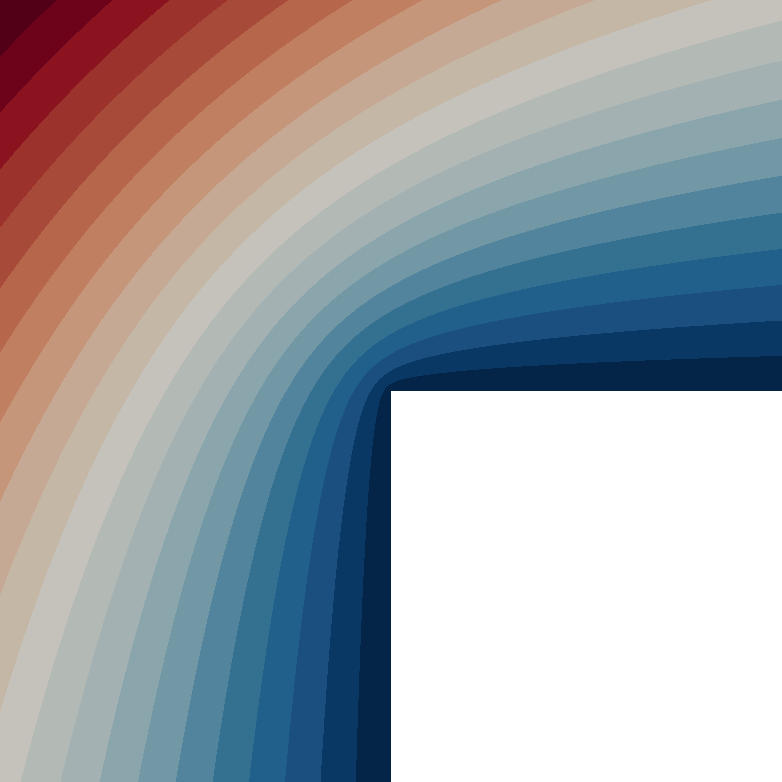
\includegraphics[width=0.499\textwidth]{solution}\hfill
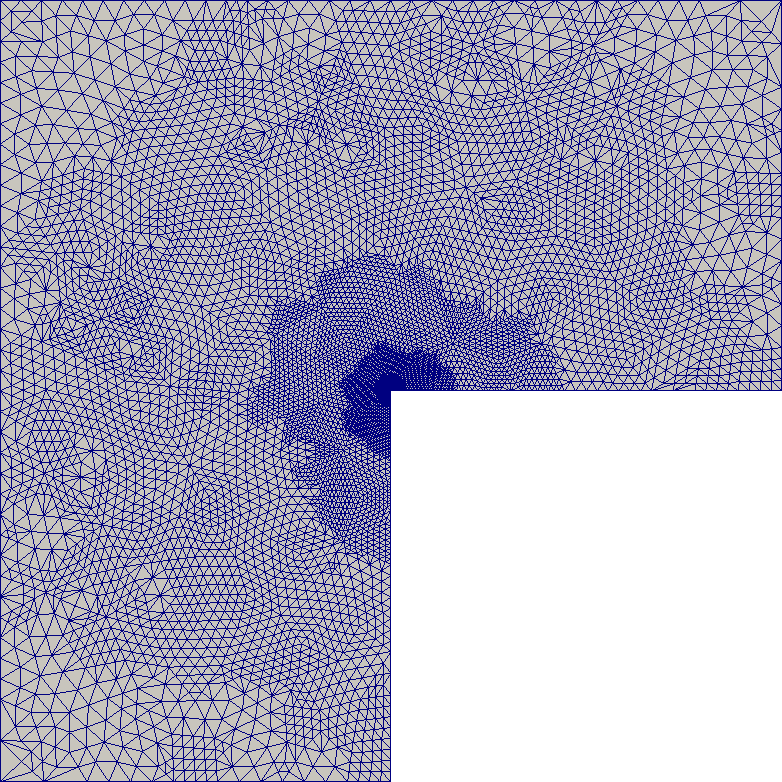
\includegraphics[width=0.499\textwidth]{refined_mesh}
\end{center}
\caption{Solution on the finest mesh and underlying elements. The colormap
  for the solution uses discrete intervals to make the large gradients in
  the reentrant corner visible. Refinement has mainly occurred in this area,
  as can be seen on the right.}
  \label{fig:results}
\end{figure}

\section{Outlook}

The interested reader can proceed in different directions from here.
The more obvious things are:
\begin{itemize}
\item Change the fraction of elements that is refined in each iteration
  and compare the resulting meshes, error estimates and convergence
  behavior.
\item Switch to a different grid manager and examine the resulting meshes
  for similarities and differences.
\item Test the reliability of the error estimate when a nonlinear function
  is used for $q$, or use a different right hand side $f$.
\end{itemize}

% bibtex bibliography
\bibliographystyle{plain}
\bibliography{tutorial05}

\end{document}
